\documentclass{beamer}

\usepackage{graphicx}
\usepackage{algorithm2e}
\usepackage{textpos}
\usepackage{verbatim}

\setbeamertemplate{caption}[numbered]

\usepackage{tikz}
\usetikzlibrary{shapes.geometric}
\usetikzlibrary{arrows,shapes,trees}
\usetikzlibrary{calc,shapes.multipart,chains,arrows}

\usepackage[dvipsnames]{xcolor}
\definecolor{pblue}{rgb}{0.13,0.13,1}
\definecolor{pgreen}{rgb}{0,0.5,0}
\definecolor{pred}{rgb}{0.9,0,0}
\definecolor{pgrey}{rgb}{0.46,0.45,0.48}

\usepackage{listings}
\lstset{language=Java,
    showspaces=false,
    showtabs=false,
    breaklines=true,
    showstringspaces=false,
    breakatwhitespace=true,
    commentstyle=\color{pgreen},
    keywordstyle=\color{pblue},
    stringstyle=\color{pred},
    basicstyle=\footnotesize,
    colframe=white!75!black,
    moredelim=[is][\textcolor{pgrey}]{\%\%}{\%\%}
}

\pgfdeclareshape{plain triangle}{
    \nodeparts{}
    \anchor{center}{\pgfpoint{0cm}{0cm}}
    \behindbackgroundpath{
		\path [draw,dashed] (0,0) -- (.5,-1) -- (-0.5,-1) -- cycle;
   }
   \pgfsetcolor{red}
}

\pgfdeclareshape{blue triangle}{
    \nodeparts{}
    \anchor{center}{\pgfpoint{0cm}{0cm}}
    \behindbackgroundpath{
		\path [draw,dashed, fill=blue] (0,0) -- (.5,-1) -- (-0.5,-1) -- cycle;
   }
   \pgfsetcolor{red}
}

\pgfdeclareshape{red triangle}{
    \nodeparts{}
    \anchor{center}{\pgfpoint{0cm}{0cm}}
    \behindbackgroundpath{
		\path [draw,dashed, fill=red] (0,0) -- (.5,-1) -- (-0.5,-1) -- cycle;
   }
   \pgfsetcolor{red}
}
\usetheme{Madrid}
\useoutertheme{miniframes} % Alternatively: miniframes, infolines, split



% Setup the university's color pallette
\definecolor{UIUCorange}{RGB}{19, 41, 75} % UBC Blue (primary)
\definecolor{UIUCblue}{RGB}{232, 74, 39} % UBC Grey (secondary)


\setbeamercolor{palette primary}{bg=UIUCorange,fg=white}
\setbeamercolor{palette secondary}{bg=UIUCblue,fg=white}
\setbeamercolor{palette tertiary}{bg=UIUCblue,fg=white}
\setbeamercolor{palette quaternary}{bg=UIUCblue,fg=white}
\setbeamercolor{structure}{fg=UIUCorange} % itemize, enumerate, etc
\setbeamercolor{section in toc}{fg=UIUCblue} % TOC sections

\setbeamercolor{subsection in head/foot}{bg=UIUCorange,fg=UIUCblue}
\setbeamercolor{subsection in head/foot}{bg=UIUCorange,fg=UIUCblue}

\usepackage[utf8]{inputenc}


%Information to be included in the title page:
\title{\textbf{Trees}}
\author{\textbf{Author}}
\institute[\textbf{UIUC}]{\textbf{University of Illinois Urbana-Champaign}}
\date{\textbf{Date}}

\setbeamertemplate{title page}[default][colsep=-4bp,rounded=true]
\addtobeamertemplate{title page}{\vspace{3\baselineskip}}{}
\addtobeamertemplate{title page}{
    \begin{textblock*}{\paperwidth}(-1.0em, -1.2em)
        \includegraphics[width=\paperwidth, height=\paperheight]{imgs/uiuc.jpg}
    \end{textblock*} 
}{}

\begin{document}

\pgfdeclarelayer{background}
\pgfsetlayers{background,main}

\tikzstyle{vertex}=[circle,fill=black!25,minimum size=20pt,inner sep=0pt]
\tikzstyle{selected vertex} = [vertex, fill=orange!24]
\tikzstyle{edge} = [draw,thick,-]
\tikzstyle{weight} = [font=\small]
\tikzstyle{selected edge} = [draw,line width=5pt,-,blue!50]
\tikzstyle{ignored edge} = [draw,line width=5pt,-,black!20]


\frame{\titlepage}

\section{Objectives}
\begin{frame}
	\frametitle{Objectives}
    \centering
    \begin{itemize}
		\item Identify the core componenets of trees in general
		\item Cover the implementation of Binary Tree nodes and traversal algorithms.
		\item Identify the motivations for using Binary Search Trees (BST)
		\item Cover the implementation of the following BST methods:
		\begin{itemize}
			\item Search
			\item Adding a node
			\item Removing a node
		\end{itemize}
    \end{itemize}
\end{frame}


\section{Trees in General}

\begin{frame}
    \frametitle{Unifying Structure}
    \begin{minipage}{0.49\textwidth}
        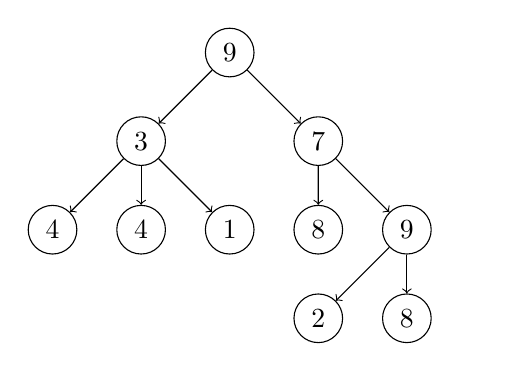
\begin{tikzpicture}[level distance=1.5cm,
            level 1/.style={sibling distance=3cm},
            level 2/.style={sibling distance=1.5cm},
            every node/.style = {minimum width = 1.0em, draw, circle},
            scale=0.75
            ]
            \node {9}
                child {node {3}
                    child {node {4} edge from parent[->]}
                    child {node {4} edge from parent[->]}
                    child {node {1} edge from parent[->]}
                    edge from parent[->]
                }
                child {node {7}
                    child {edge from parent[draw = none]}
                    child {node {8} edge from parent[->]}
                    child {node {9} 
                        child {node {2} edge from parent[->]}
                        child {node {8} edge from parent[->]}
                        child {edge from parent[draw = none]}
                        edge from parent[->]
                    }
                    edge from parent[->]
                };
        \end{tikzpicture}
    \end{minipage}
    \begin{minipage}{0.49\textwidth}
		Trees have the following general, properties:
        \begin{itemize}
            \item \textit{Directed:} Like a singly linked list a node does not have a reference to its parent.
            \item \textit{Acyclic:} There are no ``circles'' of reference in the tree. 
            \item A collection of nodes with:
                \begin{itemize}
                    \item Some data (generally)
                    \item The ability to reference child nodes
                \end{itemize}
        \end{itemize}
    \end{minipage}
\end{frame}

\begin{frame}
    \frametitle{Tree Terminology: Structural}
    \begin{minipage}{0.49\textwidth}
        \begin{itemize}
            \item \textit{root} (red)
            \item \textit{branch}  (blue)
            \item \textit{leaf}  (green)
        \end{itemize}
    \end{minipage}
    \hfill
    \begin{minipage}{0.49\textwidth}
        \begin{tikzpicture}[level distance=1.5cm,
            level 1/.style={sibling distance=3cm},
            level 2/.style={sibling distance=1.5cm},
            every node/.style = {minimum width = 1.0em, draw, circle},
            scale=0.75
            ] \node[fill=!10!red] {9}
                child {node[fill=!10!blue] {3}
                    child {node[fill=!10!green] {4} edge from parent[->]}
                    child {node[fill=!10!green] {4} edge from parent[->]}
                    child {node[fill=!10!green] {1} edge from parent[->]}
                    edge from parent[->]
                }
                child {node[fill=!10!blue] {7} 
                    child {edge from parent[draw = none]}
                    child {node[fill=!10!green] {8} edge from parent[->]}
                    child {node[fill=!10!blue] {9} 
                        child {node[fill=!10!green] {2} edge from parent[->]}
                        child {node[fill=!10!green] {8} edge from parent[->]}
                        child {edge from parent[draw = none]}
                        edge from parent[->]
                    }
                    edge from parent[->]
                };
        \end{tikzpicture}
    \end{minipage}
\end{frame}

\begin{frame}
    \frametitle{Tree Terminology: Relationship Based}
    \begin{minipage}{0.49\textwidth}
        Terms based on relationships between nodes
        \begin{itemize}
            \item \textit{parent} (blue)
            \item \textit{child/sibling} (green)
        \end{itemize}
        The blue node has three \textit{child} nodes (green) and, as a result, the green nodes are siblings.
    \end{minipage}
    \hfill
    \begin{minipage}{0.45\textwidth}
        \begin{tikzpicture}[level distance=1.5cm,
            level 1/.style={sibling distance=3cm},
            level 2/.style={sibling distance=1.5cm},
            every node/.style = {minimum width = 1.0em, draw, circle},
            scale=0.75
            ]
            \node {9}
                child {node[fill=!10!blue] {3}
                    child {node[fill=!10!green] {4} edge from parent[->]}
                    child {node[fill=!10!green] {4} edge from parent[->]}
                    child {node[fill=!10!green] {1} edge from parent[->]}
                    edge from parent[->]
                }
                child {node {7} 
                    child {edge from parent[draw = none]}
                    child {node {8} edge from parent[->]}
                    child {node {9} 
                        child {node {2} edge from parent[->]}
                        child {node {8} edge from parent[->]}
                        child {edge from parent[draw = none]}
                        edge from parent[->]
                    }
                    edge from parent[->]
                };
        \end{tikzpicture}
    \end{minipage}
\end{frame}

\begin{frame}
    \frametitle{Tree Terminology: Subtrees}
	\begin{minipage}{0.4\textwidth}
		\centering
		\begin{tikzpicture}[level distance=1.5cm,
			level 1/.style={sibling distance=3cm},
			level 2/.style={sibling distance=1.5cm},
			every node/.style = {minimum width = 1.75em, draw, circle},
			scale=0.75
			]
			\node {9}
				child {node[fill=!10!red] {1}
					child {node[fill=!10!red] {3} edge from parent[->]}
					child {edge from parent[draw = none]}
					edge from parent[->]
				}
				child {node[fill=!10!blue] {8} 
					child {node[fill=!10!blue]{7} edge from parent[->]}
					child {node[fill=!10!blue]{9} 
						edge from parent[->]
					}
					edge from parent[->]
				};
		\end{tikzpicture}
	\end{minipage}
	\hfill
	\textrightarrow
	\hfill
	\begin{minipage}{0.4\textwidth}
		\centering
		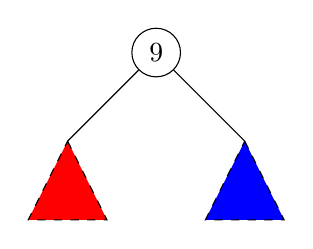
\begin{tikzpicture}[level distance=1.5cm,
			level 1/.style={sibling distance=3cm},
			level 2/.style={sibling distance=1.5cm},
			every node/.style = {minimum width = 1.75em, draw, circle},
			scale=0.75
			] 
			\node {9}
				child{node[red triangle] {} }
				child{node[blue triangle] {} };
		\end{tikzpicture}
	\end{minipage}
\end{frame}

\section{Binary Trees}

\begin{frame}[fragile]
    \frametitle{Binary Tree Structure}
    \begin{minipage}{0.59\textwidth}
        \textbf{Binary Tree:} Just a tree where each node has \textit{at most two children}.
        \begin{lstlisting}[autogobble]
class IntTree{
    static class IntTreeNode{
        int data;
        IntTreeNode left;
        IntTreeNode right;

        IntTreeNode(int. data){
            //..
        }
    }

    IntTreeNode root;
    //..
}
        \end{lstlisting}
    \end{minipage}
    \hfill
    \begin{minipage}{0.39\textwidth}
        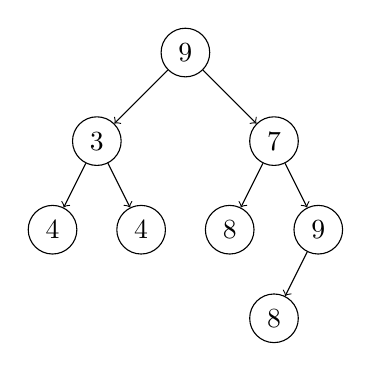
\begin{tikzpicture}[level distance=1.5cm,
            level 1/.style={sibling distance=3cm},
            level 2/.style={sibling distance=1.5cm},
            every node/.style = {minimum width = 1.0em, draw, circle},
            scale=0.75
            ]
            \node {9}
                child {node {3}
                    child {node {4} edge from parent[->]}
                    child {node {4} edge from parent[->]}
                    edge from parent[->]
                }
                child {node {7} 
                    child {node {8} edge from parent[->]}
                    child {node {9} 
                        child {node {8} edge from parent[->]}
                        child {edge from parent[draw = none]}
                        edge from parent[->]
                    }
                    edge from parent[->]
                };
        \end{tikzpicture}
    \end{minipage}
\end{frame}

\begin{frame}[fragile]
    \frametitle{Binary Tree Structure}
    \begin{minipage}{0.59\textwidth}
        \textbf{Binary Tree:} Just a tree where each node has \textit{at most two children}.
        \begin{lstlisting}[language=Java, autogobble]
class GenericTree<E>
    class GenericTreeNode<E>{
        E data;
        GenericTreeNode<E> left;
        GenericTreeNode<E> right;

        GenericTreeNode(E data){
            //..
        }
    }

    GenericTreeNode<E> root;
    //..
}
        \end{lstlisting}
    \end{minipage}
    \hfill
    \begin{minipage}{0.39\textwidth}
        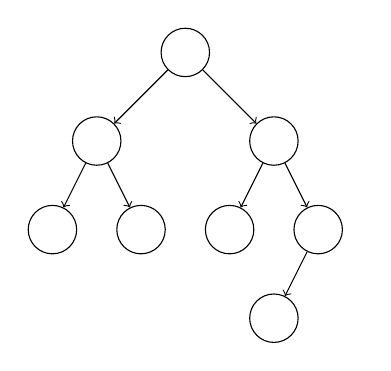
\begin{tikzpicture}[level distance=1.5cm,
            level 1/.style={sibling distance=3cm},
            level 2/.style={sibling distance=1.5cm},
            every node/.style = {minimum width = 1.75em, draw, circle},
            scale=0.75
            ]
            \node {}
                child {node {}
                    child {node {} edge from parent[->]}
                    child {node {} edge from parent[->]}
                    edge from parent[->]
                }
                child {node {} 
                    child {node {} edge from parent[->]}
                    child {node {} 
                        child {node {} edge from parent[->]}
                        child {edge from parent[draw = none]}
                        edge from parent[->]
                    }
                    edge from parent[->]
                };
        \end{tikzpicture}
    \end{minipage}
\end{frame}

\begin{frame}[fragile]
    \frametitle{Binary Tree: Manual Construction }
    \begin{minipage}{0.69\textwidth}
        \begin{lstlisting}[language=Java, autogobble, basicstyle=\scriptsize]
class Tree{

    IntTreeNode root:

    Tree(){
        root = new IntTreeNode(4);
        root.left = new IntTreeNode(1);
        root.left.left = new IntTreeNode(3);
        root.right = new IntTreeNode(8);
        root.right.left = new IntTreeNode(7);
        root.right.right = new IntTreeNode(9);
    }

    public static void main(String[] args){
        Tree myTree = new Tree();
    }
}
        \end{lstlisting}
    \end{minipage}
    \hfill
    \begin{minipage}{0.29\textwidth}
        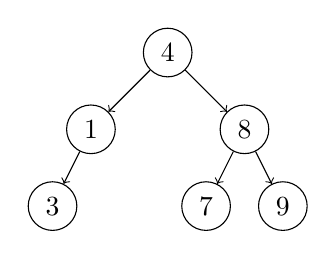
\begin{tikzpicture}[level distance=1.5cm,
            level 1/.style={sibling distance=3cm},
            level 2/.style={sibling distance=1.5cm},
            every node/.style = {minimum width = 1.75em, draw, circle},
            scale=0.65
            ]
            \node {4}
                child {node {1}
                    child {node {3} edge from parent[->]}
                    child {edge from parent[draw = none]}
                    edge from parent[->]
                }
                child {node {8} 
                    child {node {7} edge from parent[->]}
                    child {node {9} 
                        edge from parent[->]
                    }
                    edge from parent[->]
                };
        \end{tikzpicture}
    \end{minipage}
\end{frame}


\section{Binary Tree Algorithms}


\begin{frame}
	\frametitle{Recursive Traversal Algorithms}
	\begin{minipage}{0.32\textwidth}
		\scriptsize
		\centering
		\begin{algorithm}[H]
			%\algsetup{linenosize=\tiny}
			\DontPrintSemicolon
			\SetKwFunction{FInorder}{Inorder}
			\SetKwProg{Fn}{Function}{}{\KwRet}
			\Fn{\FInorder{curr}}{
				\If{curr is null}{
					return\;
				}
				Inorder(node.left)\;
				print(node)\;
				Inorder(node.right)\;
			}
		\end{algorithm}
		\textbf{Inorder:} left, visit, right
	\end{minipage}
	\pause
	\begin{minipage}{0.32\textwidth}
		\scriptsize
		\centering
		\begin{algorithm}[H]
			\DontPrintSemicolon
			\SetKwFunction{FPreorder}{Preorder}
			\SetKwProg{Fn}{Function}{}{\KwRet}
			\Fn{\FPreorder{curr}}{
				\If{curr is null}{
					return\;
				}
				print(node)\;
				Preorder(node.left)\;
				Preorder(node.right)\;
			}
		\end{algorithm}
		\textbf{Preorder:} visit, left, right
	\end{minipage}
	\pause
	\begin{minipage}{0.32\textwidth}
		\scriptsize
		\centering
		\begin{algorithm}[H]
			\DontPrintSemicolon
			\SetKwFunction{FPostorder}{Postorder}
			\SetKwProg{Fn}{Function}{}{\KwRet}
			\Fn{\FPostorder{curr}}{
				\If{curr is null}{
					return\;
				}
				Postorder(node.left)\;
				Postorder(node.right)\;
				print(node)\;
			}
		\end{algorithm}
		\textbf{Postorder:} left, right, visit
	\end{minipage}
	\pause
	\vfill
	\textbf{Left, right, visit!? What does it mean!?}
	\vfill
\end{frame}

\begin{frame}[fragile]
	\frametitle{Traversals: Recall Subtrees}
	\begin{minipage}{0.4\textwidth}
		\centering
		\begin{tikzpicture}[level distance=1.5cm,
			level 1/.style={sibling distance=3cm},
			level 2/.style={sibling distance=1.5cm},
			every node/.style = {minimum width = 1.75em, draw, circle},
			scale=0.75
			]
			\node {9}
				child {node[fill=!10!red] {1}
					child {node[fill=!10!red] {3} edge from parent[->]}
					child {edge from parent[draw = none]}
					edge from parent[->]
				}
				child {node[fill=!10!blue] {8} 
					child {node[fill=!10!blue]{7} edge from parent[->]}
					child {node[fill=!10!blue]{9} 
						edge from parent[->]
					}
					edge from parent[->]
				};
		\end{tikzpicture}
	\end{minipage}
	\hfill
	\textrightarrow
	\hfill
	\begin{minipage}{0.4\textwidth}
		\centering
		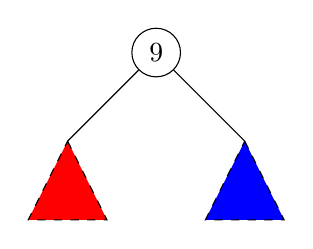
\begin{tikzpicture}[level distance=1.5cm,
			level 1/.style={sibling distance=3cm},
			level 2/.style={sibling distance=1.5cm},
			every node/.style = {minimum width = 1.75em, draw, circle},
			scale=0.75
			] 
			\node {9}
				child{node[red triangle] {} }
				child{node[blue triangle] {} };
		\end{tikzpicture}
	\end{minipage}
\end{frame}


%
% Preorder Traversals: 
%

\begin{frame}
    \frametitle{Traversals: Preorder Intuition}
	\vfill
	\begin{minipage}{0.32\textwidth}
		\centering
		\begin{tikzpicture}[level distance=1.5cm,
			level 1/.style={sibling distance=3cm},
			every node/.style = {minimum width = 1.75em, draw, circle},
			scale=0.5
			] 
			\node[fill=!10!red] {A}
				child{node[plain triangle] {} }
				child{node[plain triangle] {} };
		\end{tikzpicture}
	\end{minipage}
	\hfill
	\begin{minipage}{0.32\textwidth}
		\centering
		\begin{tikzpicture}[level distance=1.5cm,
			level 1/.style={sibling distance=3cm},
			every node/.style = {minimum width = 1.75em, draw, circle},
			scale=0.5
			] 
			\node[fill=!10!red] {A}
				child{node[red triangle] {} }
				child{node[plain triangle] {} };
		\end{tikzpicture}
	\end{minipage}
	\hfill
	\begin{minipage}{0.32\textwidth}
		\centering
		\begin{tikzpicture}[level distance=1.5cm,
			level 1/.style={sibling distance=3cm},
			every node/.style = {minimum width = 1.75em, draw, circle},
			scale=0.5
			] 
			\node[fill=!10!red] {A}
				child{node[red triangle] {} }
				child{node[red triangle] {} };
		\end{tikzpicture}
	\end{minipage}
	\vfill
	For a given node A visit that node immediatly upon encountering it and then traverse to it's left and right subtrees
	\vfill
\end{frame}

\begin{frame}
    \frametitle{Traversals}
    \centering
    \begin{minipage}{0.49\textwidth}
        \begin{algorithm}[H]
            \DontPrintSemicolon
            \SetKwFunction{FPreorder}{Preorder}
            \SetKwProg{Fn}{Function}{}{\KwRet}
            \Fn{\FPreorder{curr}}{
                \If{curr is null}{
                    return\;
                }
                print(curr)\;
                Preorder(curr.left)\;
                Preorder(curr.right)\;
            }
        \end{algorithm}
    \end{minipage}
    \hfill
    \begin{minipage}{0.49\textwidth}
        \begin{figure}[H]
            \centering
            \begin{tikzpicture}[level distance=1.5cm,
                level 1/.style={sibling distance=3cm},
                level 2/.style={sibling distance=1.5cm},
                every node/.style = {minimum width = 1.0em, draw, circle},
                scale=0.75
                ]
                \node (A) {9}
                    child {node (B) {3}
                        child {node (D) {4} edge from parent[->]}
                        child {node (E) {4} edge from parent[->]}
                        edge from parent[->]
                    }
                    child {node (C) {7} 
                        child {edge from parent[draw = none]}
                        child {node (F) {9} 
                            child {node (G) {2} edge from parent[->]}
                            child {node (H) {8} edge from parent[->]}
                            edge from parent[->]
                        }
                        edge from parent[->]
                    };

                \begin{pgfonlayer}{background}
                    \foreach \vertex in {A, B, D, E, C, F, G, H}
                    \pause
                    \node[fill=!10!red] at (\vertex) {};
                \end{pgfonlayer}
            \end{tikzpicture}
        \end{figure}
    \end{minipage}
\end{frame}

%\begin{frame}
%    \frametitle{Traversals Activity: Find the Preorder Traversal}
%    \centering
%    \begin{minipage}{0.49\textwidth}
%        \begin{figure}[H]
%            \centering
%            \begin{tikzpicture}[level distance=1.5cm,
%                level 1/.style={sibling distance=3cm},
%                level 2/.style={sibling distance=1.5cm},
%                every node/.style = {minimum width = 1.0em, draw, circle},
%                scale=0.75
%                ]
%                \node (A) {6}
%                    child {node (B) {1}
%                        child {node (E) {8} edge from parent[->]}
%                        child {node (F) {9} 
%                            child {node (G) {2} edge from parent[->]}
%                            child {node (H) {8} edge from parent[->]}
%                            edge from parent[->]
%                        }
%                        edge from parent[->]
%                    }
%                    child {node (C) {7} 
%                        child {edge from parent[draw = none]}
%                        child {
%                            edge from parent[draw = none]
%                        }
%                        edge from parent[->]
%                    };
%            \end{tikzpicture}
%        \end{figure}
%    \end{minipage}
%    \hfill
%    \begin{minipage}{0.49\textwidth}
%        \begin{algorithm}[H]
%            \DontPrintSemicolon
%            \SetKwFunction{FPreorder}{Preorder}
%            \SetKwProg{Fn}{Function}{}{\KwRet}
%            \Fn{\FPreorder{curr}}{
%                \If{curr is null}{
%                    return\;
%                }
%                print(node)\;
%                Preorder(node.left)\;
%                Preorder(node.right)\;
%            }
%        \end{algorithm}
%        \vspace{0.5cm}\\
%        \pause
%    \end{minipage}
%
%\end{frame}


%
% Inorder Traversals: 
%

\begin{frame}
    \frametitle{Traversals: Inorder Intuition}
	\vfill
	\begin{minipage}{0.32\textwidth}
		\centering
		\begin{tikzpicture}[level distance=1.5cm,
			level 1/.style={sibling distance=3cm},
			every node/.style = {minimum width = 1.75em, draw, circle},
			scale=0.5
			] 
			\node[fill=!10!blue] {A}
				child{node[red triangle] {} }
				child{node[plain triangle] {} };
		\end{tikzpicture}
	\end{minipage}
	\hfill
	\begin{minipage}{0.32\textwidth}
		\centering
		\begin{tikzpicture}[level distance=1.5cm,
			level 1/.style={sibling distance=3cm},
			every node/.style = {minimum width = 1.75em, draw, circle},
			scale=0.5
			] 
			\node[fill=!10!red] {A}
				child{node[red triangle] {} }
				child{node[plain triangle] {} };
		\end{tikzpicture}
	\end{minipage}
	\hfill
	\begin{minipage}{0.32\textwidth}
		\centering
		\begin{tikzpicture}[level distance=1.5cm,
			level 1/.style={sibling distance=3cm},
			every node/.style = {minimum width = 1.75em, draw, circle},
			scale=0.5
			] 
			\node[fill=!10!red] {A}
				child{node[red triangle] {} }
				child{node[red triangle] {} };
		\end{tikzpicture}
	\end{minipage}
	\vfill
	For a given node A, all nodes in A's left subtree must be visited before we visit A.
	\vfill
\end{frame}

\begin{frame}
    \frametitle{Traversals}
    \begin{minipage}{0.49\textwidth}
        \begin{algorithm}[H]
            \DontPrintSemicolon
            \SetKwFunction{FInorder}{Inorder}
            \SetKwProg{Fn}{Function}{}{\KwRet}
            \Fn{\FInorder{curr}}{
                \If{curr is null}{
                    return\;
                }
                Inorder(curr.left)\;
                print(curr)\;
                Inorder(curr.right)\;
            }
        \end{algorithm}\\
        \vspace{0.25cm}\\
    \end{minipage}
    \hfill
    \begin{minipage}{0.49\textwidth}
        \begin{figure}[H]
            \centering
            \begin{tikzpicture}[level distance=1.5cm,
                level 1/.style={sibling distance=3cm},
                level 2/.style={sibling distance=1.5cm},
                every node/.style = {minimum width = 1.0em, draw, circle},
                scale=0.75
                ]
                \node (A) {9}
                    child {node (B) {3}
                        child {node (D) {4} edge from parent[->]}
                        child {node (E) {4} edge from parent[->]}
                        edge from parent[->]
                    }
                    child {node (C) {7} 
                        child {edge from parent[draw = none]}
                        child {node (F) {9} 
                            child {node (G) {2} edge from parent[->]}
                            child {node (H) {8} edge from parent[->]}
                            edge from parent[->]
                        }
                        edge from parent[->]
                    };

                \begin{pgfonlayer}{background}
                    \foreach \vertex/ \color in {A/blue, B/blue, D/blue, D/red, 
                        B/red, 
                        E/blue, E/red,
                        A/red, 
                        C/blue, C/red,
                        F/blue, G/blue, G/red,
                        H/blue, H/red,
                    F/red}
                    \pause
                    \node[fill=!10!\color] at (\vertex) {};
                \end{pgfonlayer}
            \end{tikzpicture}
        \end{figure}
    \end{minipage}
\end{frame}

%\begin{frame}
%    \frametitle{Traversals Activity: Find the Inorder Traversal}
%    \centering
%    \begin{minipage}{0.49\textwidth}
%        \begin{figure}[H]
%            \centering
%            \begin{tikzpicture}[level distance=1.5cm,
%                level 1/.style={sibling distance=3cm},
%                level 2/.style={sibling distance=1.5cm},
%                every node/.style = {minimum width = 1.0em, draw, circle},
%                scale=0.75
%                ]
%                \node (A) {6}
%                    child {node (B) {1}
%                        child {node (E) {8} edge from parent[->]}
%                        child {node (F) {9} 
%                            child {node (G) {2} edge from parent[->]}
%                            child {node (H) {8} edge from parent[->]}
%                            edge from parent[->]
%                        }
%                        edge from parent[->]
%                    }
%                    child {node (C) {7} 
%                        child {edge from parent[draw = none]}
%                        child {
%                            edge from parent[draw = none]
%                        }
%                        edge from parent[->]
%                    };
%            \end{tikzpicture}
%        \end{figure}
%    \end{minipage}
%    \hfill
%    \begin{minipage}{0.49\textwidth}
%        \begin{algorithm}[H]
%            \DontPrintSemicolon
%            \SetKwFunction{FInorder}{Inorder}
%            \SetKwProg{Fn}{Function}{}{\KwRet}
%            \Fn{\FInorder{curr}}{
%                \If{curr is null}{
%                    return\;
%                }
%                Inorder(node.left)\;
%                print(node)\;
%                Inorder(node.right)\;
%            }
%        \end{algorithm}\\
%        \vspace{0.5cm}\\
%    \end{minipage}
%
%\end{frame}



%
% Postorder Traversals: 
%

\begin{frame}
    \frametitle{Traversals: Postorder Intuition}
	\vfill
	\begin{minipage}{0.32\textwidth}
		\centering
		\begin{tikzpicture}[level distance=1.5cm,
			level 1/.style={sibling distance=3cm},
			every node/.style = {minimum width = 1.75em, draw, circle},
			scale=0.5
			] 
			\node[fill=!10!blue] {A}
				child{node[red triangle] {} }
				child{node[plain triangle] {} };
		\end{tikzpicture}
	\end{minipage}
	\hfill
	\begin{minipage}{0.32\textwidth}
		\centering
		\begin{tikzpicture}[level distance=1.5cm,
			level 1/.style={sibling distance=3cm},
			every node/.style = {minimum width = 1.75em, draw, circle},
			scale=0.5
			] 
			\node[fill=!10!blue] {A}
				child{node[red triangle] {} }
				child{node[red triangle] {} };
		\end{tikzpicture}
	\end{minipage}
	\hfill
	\begin{minipage}{0.32\textwidth}
		\centering
		\begin{tikzpicture}[level distance=1.5cm,
			level 1/.style={sibling distance=3cm},
			every node/.style = {minimum width = 1.75em, draw, circle},
			scale=0.5
			] 
			\node[fill=!10!red] {A}
				child{node[red triangle] {} }
				child{node[red triangle] {} };
		\end{tikzpicture}
	\end{minipage}
	\vfill
	For a given node A, all of the nodes in A's left and right subtrees must be
	visited before A can be visited.
	\vfill
\end{frame}


\begin{frame}
    \frametitle{Traversals: Postorder}
    \begin{minipage}{0.49\textwidth}
        \begin{algorithm}[H]
            \DontPrintSemicolon
            \SetKwFunction{FPostorder}{Postorder}
            \SetKwProg{Fn}{Function}{}{\KwRet}
            \Fn{\FPostorder{curr}}{
                \If{curr is null}{
                    return\;
                }
                Postorder(curr.left)\;
                Postorder(curr.right)\;
                print(node)\;
            }
        \end{algorithm}
    \end{minipage}
    \hfill
    \begin{minipage}{0.49\textwidth}
        \begin{figure}[H]
            \centering
            \begin{tikzpicture}[level distance=1.5cm,
                level 1/.style={sibling distance=3cm},
                level 2/.style={sibling distance=1.5cm},
                every node/.style = {minimum width = 1.0em, draw, circle},
                scale=0.75
                ]
                \node (A) {9}
                    child {node (B) {3}
                        child {node (D) {4} edge from parent[->]}
                        child {node (E) {4} edge from parent[->]}
                        edge from parent[->]
                    }
                    child {node (C) {7} 
                        child {edge from parent[draw = none]}
                        child {node (F) {9} 
                            child {node (G) {2} edge from parent[->]}
                            child {node (H) {8} edge from parent[->]}
                            edge from parent[->]
                        }
                        edge from parent[->]
                    };

                \begin{pgfonlayer}{background}
                    \foreach \vertex/ \color in {A/blue, B/blue, D/blue, D/red, 
                        E/blue, E/red,
                        B/red, 
                        C/blue, 
                        F/blue, G/blue, G/red,
                        H/blue, H/red,
                    F/red, C/red, A/red}
                    \pause
                    \node[fill=!10!\color] at (\vertex) {};
                \end{pgfonlayer}
            \end{tikzpicture}
        \end{figure}
    \end{minipage}
\end{frame}

%\begin{frame}
%    \frametitle{Traversals Activity: Find the Postorder Traversal}
%    \centering
%    \begin{minipage}{0.49\textwidth}
%        \begin{figure}[H]
%            \centering
%            \begin{tikzpicture}[level distance=1.5cm,
%                level 1/.style={sibling distance=3cm},
%                level 2/.style={sibling distance=1.5cm},
%                every node/.style = {minimum width = 1.0em, draw, circle},
%                scale=0.75
%                ]
%                \node (A) {6}
%                    child {node (B) {1}
%                        child {node (E) {8} edge from parent[->]}
%                        child {node (F) {9} 
%                            child {node (G) {2} edge from parent[->]}
%                            child {node (H) {8} edge from parent[->]}
%                            edge from parent[->]
%                        }
%                        edge from parent[->]
%                    }
%                    child {node (C) {7} 
%                        child {edge from parent[draw = none]}
%                        child {
%                            edge from parent[draw = none]
%                        }
%                        edge from parent[->]
%                    };
%            \end{tikzpicture}
%        \end{figure}
%    \end{minipage}
%    \hfill
%    \begin{minipage}{0.49\textwidth}
%        \begin{algorithm}[H]
%            \DontPrintSemicolon
%            \SetKwFunction{FPostorder}{Postorder}
%            \SetKwProg{Fn}{Function}{}{\KwRet}
%            \Fn{\FPostorder{curr}}{
%                \If{curr is null}{
%                    return\;
%                }
%                Postorder(node.left)\;
%                Postorder(node.right)\;
%                print(node)\;
%            }
%        \end{algorithm}\\
%        \vspace{0.5cm}\\
%        \pause
%    \end{minipage}
%\end{frame}

\section{Binary Search Tree}


\begin{frame}[fragile]
	\frametitle{Binary Search Tree: Structure}
	\textbf{Binary Search Tree:} A tree where: 
	\begin{enumerate}[1]
		\item each node has \textit{at most two children}.
		\item the value of a given node is greater than the value of every node in it's left subtree.
		\item the value of a given node is less than the value of every node in it's right subtree.
	\end{enumerate}
	\vfill
	\begin{figure}
	\centering
	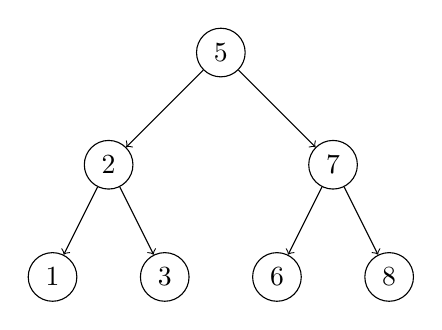
\begin{tikzpicture}[level distance=1.5cm,
		level 1/.style={sibling distance=3cm},
		level 2/.style={sibling distance=1.5cm},
		every node/.style = {minimum width = 1.75em, draw, circle},
		scale=0.95
		]
		\node {5}
			child {node {2}
				child {node {1} edge from parent[->]}
				child {node {3} edge from parent[->]}
				edge from parent[->]
			}
			child {node {7} 
				child {node {6} edge from parent[->]}
				child {node {8} edge from parent[->]}
				edge from parent[->]
			};
	\end{tikzpicture}
	\end{figure}
\end{frame}

\section{Binary Search Tree Algorithms}

\begin{frame}[fragile]
	\frametitle{Binary Tree: Terms and Basic Operations}
    \vfill
    \begin{minipage}{0.49\textwidth}
    \begin{algorithm}[H]
        \DontPrintSemicolon
        \SetKwFunction{FMinimum}{Minimum}
        \SetKwProg{Fn}{Function}{}{\KwRet curr\;}
        \Fn{\FMinimum{curr}}{
            \While{ curr.left $\neq$ \lstinline|null| }{
                curr = curr.left\;
            }
        }
    \end{algorithm}
    \end{minipage}
    \begin{minipage}{0.49\textwidth}
	\begin{figure}
	\centering
	\begin{tikzpicture}[level distance=1.5cm,
		level 1/.style={sibling distance=3cm},
		level 2/.style={sibling distance=1.5cm},
		every node/.style = {minimum width = 1.75em, draw, circle},
		scale=0.95
		]
		\node {5}
			child {node {2}
				child {node[fill=!10!orange] {1} edge from parent[->]}
				child {node {3} edge from parent[->]}
				edge from parent[->]
			}
			child {node {7} 
				child {node {6} edge from parent[->]}
				child {node {8} edge from parent[->]}
				edge from parent[->]
			};
	\end{tikzpicture}
	\end{figure}
    \end{minipage}
    \vfill
    \textbf{Minimum Node:} Starting at a given node $curr$, the node with the least value under $curr$ will be the leftmost node in it's left subtree.
    \vfill
\end{frame}

\begin{frame}[fragile]
	\frametitle{Binary Search Tree: Maximum Node}
    \vfill
    \begin{minipage}{0.49\textwidth}
    \begin{algorithm}[H]
        \DontPrintSemicolon
        \SetKwFunction{FMaximum}{Maximum}
        \SetKwProg{Fn}{Function}{}{\KwRet curr\;}
        \Fn{\FMaximum{curr}}{
            \While{ curr.right $\neq$ \lstinline|null| }{
                curr = curr.right\;
            }
        }
    \end{algorithm}
    \end{minipage}
    \begin{minipage}{0.49\textwidth}
	\begin{figure}
	\centering
	\begin{tikzpicture}[level distance=1.5cm,
		level 1/.style={sibling distance=3cm},
		level 2/.style={sibling distance=1.5cm},
		every node/.style = {minimum width = 1.75em, draw, circle},
		scale=0.95
		]
		\node {5}
			child {node {2}
				child {node {1} edge from parent[->]}
				child {node {3} edge from parent[->]}
				edge from parent[->]
			}
			child {node {7} 
				child {node {6} edge from parent[->]}
				child {node[fill=!10!orange] {8} edge from parent[->]}
				edge from parent[->]
			};
	\end{tikzpicture}
	\end{figure}
    \end{minipage}
    \vfill
    \textbf{Maximum Node:} Starting at a given node $curr$, the node with the greatest value under $curr$ will be the rightmost node in it's right subtree.
    \vfill
\end{frame}

%
% Successor
%
%\begin{frame}[fragile]
%    \frametitle{Binary Tree: Successor Node}
%    \vfill
%    \begin{minipage}{0.59\textwidth}
%        \begin{algorithm}[H]
%            \DontPrintSemicolon
%            \tiny
%            \SetKwFunction{FSuccessor}{Successor}
%            \SetKwProg{Fn}{Function}{}{\textbf{end}\;}
%            \Fn{\FSuccessor{root, curr}}{
%                \begingroup
%                \color{red}
%                \If{curr $=$ null}{
%                    \Return{null}\;
%                }
%                \endgroup
%                \ElseIf{curr.right $\neq$ null}{
%                    \Return{Minimum(curr.right)}\;
%                }
%                \Else{
%                    Pred $\gets$ null\;
%                    TmpRoot $\gets$ root\;
%                    \While{TmpRoot $\neq$ null AND TmpRoot.val $\neq$ curr.val}{
%                        \If{TmpRoot.val $>$ curr.val}{
%                            Pred $\gets$ TmpRoot\;
%                            TmpRoot $\gets$ TmpRoot.left\;
%                            }\Else{
%                            TmpRoot $\gets$ TmpRoot.right\;
%                        }
%                    }
%                    \Return{Pred}\;
%                }
%            }
%        \end{algorithm}
%    \end{minipage}
%    \vline
%    \hfill
%    \begin{minipage}{0.38\textwidth}
%        \textbf{Case 1:} If the root is null, then simply Return null
%    \end{minipage}
%    \vfill
%\end{frame}
%
%\begin{frame}[fragile]
%    \frametitle{Binary Tree: Successor Node}
%    \vfill
%    \begin{minipage}{0.59\textwidth}
%        \begin{algorithm}[H]
%            \DontPrintSemicolon
%            \tiny
%            \SetKwFunction{FSuccessor}{Successor}
%            \SetKwProg{Fn}{Function}{}{\textbf{end}}
%            \Fn{\FSuccessor{root, curr}}{
%                \If{curr $=$ null}{
%                    \Return{null}\;
%                }
%                \begingroup
%                \color{red}
%                \ElseIf{curr.right $\neq$ null}{
%                    \Return{Minimum(curr.right)}\;
%                }
%                \endgroup
%                \Else{
%                    Pred $\gets$ null\;
%                    TmpRoot $\gets$ root\;
%                    \While{TmpRoot $\neq$ null AND TmpRoot.val $\neq$ curr.val}{
%                        \If{TmpRoot.val $>$ curr.val}{
%                            Pred $\gets$ TmpRoot\;
%                            TmpRoot $\gets$ TmpRoot.left\;
%                            }\Else{
%                            TmpRoot $\gets$ TmpRoot.right\;
%                        }
%                    }
%                    \Return{Pred}\;
%                }
%            }
%        \end{algorithm}
%    \end{minipage}
%    \vline
%    \hfill
%    \begin{minipage}{0.38\textwidth}
%        \begin{figure}
%            \centering
%            \begin{tikzpicture}[level distance=1.5cm,
%                level 1/.style={sibling distance=3cm},
%                level 2/.style={sibling distance=1.5cm},
%                every node/.style = {minimum width = 1.75em, draw, circle},
%                scale=0.75
%                ]
%                \node[fill=!10!blue] {5}
%                    child {node {2}
%                        child {node {1} edge from parent[->]}
%                        child {node {3} edge from parent[->]}
%                        edge from parent[->]
%                    }
%                    child {node {7} 
%                        child {node[fill=!10!orange] {6} edge from parent[->]}
%                        child {node {8} edge from parent[->]}
%                        edge from parent[->]
%                    };
%            \end{tikzpicture}
%        \end{figure}
%        \textbf{Case 2:} If the root's right subtree is not empty, then the root's successor is the minimum node in it's right subtree.
%    \end{minipage}
%    \vfill
%\end{frame}
%
%\begin{frame}[fragile]
%    \frametitle{Binary Tree: Successor Node}
%    \vfill
%    \begin{minipage}{0.59\textwidth}
%        \begin{algorithm}[H]
%            \DontPrintSemicolon
%            \tiny
%            \SetKwFunction{FSuccessor}{Successor}
%            \SetKwProg{Fn}{Function}{}{\textbf{end}}
%            \Fn{\FSuccessor{root, curr}}{
%                \If{curr $=$ null}{
%                    \Return{null}\;
%                }
%                \ElseIf{curr.right $\neq$ null}{
%                    \Return{Minimum(curr.right)}\;
%                }
%                \begingroup
%                \color{red}
%                \Else{
%                    Pred $\gets$ null\;
%                    TmpRoot $\texts$ root\;
%                    \While{TmpRoot $\neq$ null AND TmpRoot.val $\neq$ curr.val}{
%                        \If{TmpRoot.val $>$ curr.val}{
%                            Pred $\gets$ TmpRoot\;
%                            TmpRoot $\gets$ TmpRoot.left\;
%                            }\Else{
%                            TmpRoot $\gets$ TmpRoot.right\;
%                        }
%                    }
%                    \Return{Pred}\;
%                }
%                \endgroup
%            }
%        \end{algorithm}
%    \end{minipage}
%    \vline
%    \hfill
%    \begin{minipage}{0.38\textwidth}
%        \begin{figure}
%            \centering
%            \begin{tikzpicture}[level distance=1.5cm,
%                level 1/.style={sibling distance=3cm},
%                level 2/.style={sibling distance=1.5cm},
%                level 3/.style={sibling distance=1.0cm},
%                every node/.style = {minimum width = 1.75em, draw, circle},
%                scale=0.7
%                ]
%                \node[fill=!10!orange] {5}
%                    child {node {3}
%                        child {edge from parent[draw = none]}
%                        child {node[fill=!10!blue] {4} edge from parent[->]}
%                        edge from parent[->]
%                    }
%                    child {node {7} 
%                        child {node {6} edge from parent[->]}
%                        child {node {9}
%                            child {node {8} edge from parent[->]}
%                            child {edge from parent[draw = none]}
%                            edge from parent[->]
%                        }
%                        edge from parent[->]
%                    };
%            \end{tikzpicture}
%        \end{figure}
%        \textbf{Case 3:} If the root's right subtree is empty, then perform a search for the successor starting at the root node of the tree.
%    \end{minipage}
%    \vfill
%\end{frame}
%
%
%%
%% Predecessor
%%
%\begin{frame}[fragile]
%    \frametitle{Binary Tree: Predecessor Node}
%    \vfill
%    \begin{minipage}{0.59\textwidth}
%        \begin{algorithm}[H]
%            \DontPrintSemicolon
%            \tiny
%            \SetKwFunction{FPredecessor}{Predecessor}
%            \SetKwProg{Fn}{Function}{}{\textbf{end}\;}
%            \Fn{\FPredecessor{root, curr}}{
%                \begingroup
%                \color{red}
%                \If{curr $=$ null}{
%                    \Return{null}\;
%                }
%                \endgroup
%                \ElseIf{curr.left $\neq$ null}{
%                    \Return{Minimum(curr.right)}\;
%                }
%                \Else{
%                    Pred $\gets$ null\;
%                    TmpRoot $\gets$ root\;
%                    \While{TmpRoot $\neq$ null AND TmpRoot.val $\neq$ curr.val}{
%                        \If{TmpRoot.val $>$ curr.val}{
%                            TmpRoot $\gets$ TmpRoot.left\;
%                            }\Else{
%                            Pred $\gets$ TmpRoot\;
%                            TmpRoot $\gets$ TmpRoot.right\;
%                        }
%                    }
%                    \Return{Pred}\;
%                }
%            }
%        \end{algorithm}
%    \end{minipage}
%    \vline
%    \hfill
%    \begin{minipage}{0.38\textwidth}
%        \textbf{Case 1:} If the root is null, then simply Return null
%    \end{minipage}
%    \vfill
%\end{frame}
%
%\begin{frame}[fragile]
%    \frametitle{Binary Tree: Predecessor Node}
%    \vfill
%    \begin{minipage}{0.59\textwidth}
%        \begin{algorithm}[H]
%            \DontPrintSemicolon
%            \tiny
%            \SetKwFunction{FPredecessor}{Predecessor}
%            \SetKwProg{Fn}{Function}{}{\textbf{end}}
%            \Fn{\FPredecessor{root, curr}}{
%                \If{curr $=$ null}{
%                    \Return{null}\;
%                }
%                \begingroup
%                \color{red}
%                \ElseIf{curr.left $\neq$ null}{
%                    \Return{Maximum(curr.left)}\;
%                }
%                \endgroup
%                \Else{
%                    Pred $\gets$ null\;
%                    TmpRoot $\gets$ root\;
%                    \While{TmpRoot $\neq$ null AND TmpRoot.val $\neq$ curr.val}{
%                        \If{TmpRoot.val $>$ curr.val}{
%                            TmpRoot $\gets$ TmpRoot.left\;
%                            }\Else{
%                            Pred $\gets$ TmpRoot\;
%                            TmpRoot $\gets$ TmpRoot.right\;
%                        }
%                    }
%                    \Return{Pred}\;
%                }
%            }
%        \end{algorithm}
%    \end{minipage}
%    \vline
%    \hfill
%    \begin{minipage}{0.38\textwidth}
%        \begin{figure}
%            \centering
%            \begin{tikzpicture}[level distance=1.5cm,
%                level 1/.style={sibling distance=3cm},
%                level 2/.style={sibling distance=1.5cm},
%                every node/.style = {minimum width = 1.75em, draw, circle},
%                scale=0.75
%                ]
%                \node[fill=!10!blue] {5}
%                    child {node {2}
%                        child {node {1} edge from parent[->]}
%                        child {node[fill=!10!orange] {3} edge from parent[->]}
%                        edge from parent[->]
%                    }
%                    child {node {7} 
%                        child {node {6} edge from parent[->]}
%                        child {node {8} edge from parent[->]}
%                        edge from parent[->]
%                    };
%            \end{tikzpicture}
%        \end{figure}
%        \textbf{Case 2:} If the root's left subtree is not empty, then the root's predecsssor is the maximum node in it's left subtree.
%    \end{minipage}
%    \vfill
%\end{frame}
%
%\begin{frame}[fragile]
%    \frametitle{Binary Tree: Predecessor Node}
%    \vfill
%    \begin{minipage}{0.59\textwidth}
%        \begin{algorithm}[H]
%            \DontPrintSemicolon
%            \tiny
%            \SetKwFunction{FPredecessor}{Predecessor}
%            \SetKwProg{Fn}{Function}{}{\textbf{end}}
%            \Fn{\FPredecessor{root, curr}}{
%                \If{curr $=$ null}{
%                    \Return{null}\;
%                }
%                \ElseIf{curr.left $\neq$ null}{
%                    \Return{Maximum(curr.left)}\;
%                }
%                \begingroup
%                \color{red}
%                \Else{
%                    Pred $\gets$ null\;
%                    TmpRoot $\texts$ root\;
%                    \While{TmpRoot $\neq$ null AND TmpRoot.val $\neq$ curr.val}{
%                        \If{TmpRoot.val $>$ curr.val}{
%                            TmpRoot $\gets$ TmpRoot.left\;
%                            }\Else{
%                            Pred $\gets$ TmpRoot\;
%                            TmpRoot $\gets$ TmpRoot.right\;
%                        }
%                    }
%                    \Return{Pred}\;
%                }
%                \endgroup
%            }
%        \end{algorithm}
%    \end{minipage}
%    \vline
%    \hfill
%    \begin{minipage}{0.38\textwidth}
%        \begin{figure}
%            \centering
%            \begin{tikzpicture}[level distance=1.5cm,
%                level 1/.style={sibling distance=3cm},
%                level 2/.style={sibling distance=1.5cm},
%                level 3/.style={sibling distance=1.0cm},
%                every node/.style = {minimum width = 1.75em, draw, circle},
%                scale=0.7
%                ]
%                \node {7}
%                    child {node[fill=!10!orange] {3}
%                        child {node {2} edge from parent[->]}
%                        child {node[fill=!10!blue] {5}
%                            child {edge from parent[draw = none]}
%                            child {node {6} edge from parent[->]}
%                            edge from parent[->]
%                        }
%                        edge from parent[->]
%                    }
%                    child {node {8} 
%                        child {edge from parent[draw = none]}
%                        child {node {9} edge from parent[->]}
%                        edge from parent[->]
%                    };
%            \end{tikzpicture}
%        \end{figure}
%        \textbf{Case 3:} If the root's left subtree is empty, then perform a search for the predecessor starting at the root node of the tree.
%    \end{minipage}
%    \vfill
%\end{frame}


%
% Search
%
\begin{frame}
    \frametitle{Binary Search Tree: Finding a Node}
    \vfill
    \begin{minipage}{0.52\textwidth}
        \centering
        \begin{algorithm}[H]
            \tiny
            \DontPrintSemicolon
            \SetKwFunction{FRecursiveSearch}{RecursiveSearch}
            \SetKwProg{Fn}{Function}{}{\KwRet\;}
            \Fn{\FRecursiveSearch{Curr, Val}}{
                \If{Curr $=$ NULL OR Val $=$ Curr.Val}{
                    \Return{curr}\;
                }
                \If{Val $<$ Curr.Val}{
                    \Return{RecursiveSearch(Curr.Left, Val)}\;
                }\Else{
                    \Return{RecursiveSearch(Curr.Right, Val)}\;
                }
            }
        \end{algorithm}
    \end{minipage}
    \hfill
    \begin{minipage}{0.47\textwidth}
        \begin{itemize}
            \item Though this can be done iteratively or recursively, both methods follow the pattern of finding and returning a reference to a node with a given value.
                \pause
            \item Searching will also form the basis for adding and removing nodes.
        \end{itemize}
    \end{minipage}
    \vfill
\end{frame}

\begin{frame}
	\frametitle{Adding a Node}
    \begin{minipage}{0.49\textwidth}
    \begin{algorithm}[H]
        \DontPrintSemicolon
        \tiny
        \SetKwFunction{FAdd}{Add}
        \SetKwProg{Fn}{Function}{}{\KwRet\;}
        \Fn{\FAdd{Data}}{
            Root = Add(Root, Data);
        }
    \end{algorithm}
    \begin{algorithm}[H]
        \DontPrintSemicolon
        \tiny
        \SetKwFunction{FAdd}{Add}
        \SetKwProg{Fn}{Function}{}{\KwRet\;}
        \Fn{\FAdd{Curr, Data}}{
            \begingroup
            \color{red}
            \If{Curr $=$ NULL}{
                \Return{TreeNode(Data)}\;
            }
            \endgroup
            \begingroup
            \color{blue}
            \ElseIf{Data $>$ Curr.Data}{
                Curr.Right $\gets$ Add(Curr.Right, Data)
            }\Else{
                Curr.Left $\gets$ Add(Curr.Left, Data)
            }
            \endgroup
            \Return{Curr}
            
        }
    \end{algorithm}
    \end{minipage}
    \hfill
    \begin{minipage}{0.49\textwidth}
        \begin{itemize}
            \item \textbf{Case 1 (red): } Curr is null so we create and return the new node.
            \item \textbf{Case 2 (blue): } Curr isn't null so we need to keep traversing according to BST rules.
        \end{itemize}
    \end{minipage}
\end{frame}


\begin{frame}
    \frametitle{Binary Search Tree: Removing a Node}
    \begin{minipage}{0.32\textwidth}
        \centering
        \vspace{0.1cm}
        \begin{figure}[H]
            \begin{tikzpicture}[level distance=1.5cm,
                level 1/.style={sibling distance=3cm},
                level 2/.style={sibling distance=1.5cm},
                every node/.style = {minimum width = 2em, draw, circle},
                scale=0.7
                ]
                \node {5}
                    child {node {3}
                        child {node {1}}
                        child {node[fill=!10!orange] {4}}
                    }
                    child {node {6}
                        child {edge from parent[draw = none]}
                        child {node {8}}
                    };
            \end{tikzpicture}
            \caption{Leaf}
            \label{fig:nodeleaf}
        \end{figure}
    \end{minipage}
    \hfill
    \begin{minipage}{0.32\textwidth}
        \centering
        \begin{figure}[H]
            \begin{tikzpicture}[level distance=1.5cm,
                level 1/.style={sibling distance=3cm},
                level 2/.style={sibling distance=1.5cm},
                every node/.style = {minimum width = 2em, draw, circle},
                scale=0.7
                ]
                \node {5}
                    child {node {3}
                        child {node {1}}
                        child {node {4}}
                    }
                    child {node[fill=!10!orange] {6}
                        child {edge from parent[draw = none]}
                        child {node {8}}
                    };
            \end{tikzpicture}
            \caption{One Subtree}
            \label{fig:nodeonechild}
        \end{figure}
    \end{minipage}
    \hfill
    \begin{minipage}{0.32\textwidth}
        \centering
        \begin{figure}[H]
            \begin{tikzpicture}[level distance=1.5cm,
                level 1/.style={sibling distance=3cm},
                level 2/.style={sibling distance=1.5cm},
                every node/.style = {minimum width = 2em, draw, circle},
                scale=0.7
                ]
                \node {5}
                    child {node[fill=!10!orange] {3}
                        child {node {1}}
                        child {node {4}}
                    }
                    child {node {6}
                        child {edge from parent[draw = none]}
                        child {node {8}}
                    };
            \end{tikzpicture}
            \caption{Two Subtrees}
            \label{fig:nodetwochildren}
        \end{figure}
    \end{minipage}
    \vspace{0.25cm}\\
    There are three cases for removing a node:
    \begin{enumerate}
        \pause
        \item The node we are removing is a leaf (Figure~\ref{fig:nodeleaf}).
        \pause
        \item The node we are removing has one subtree (Figure~\ref{fig:nodeonechild}).
        \pause
        \item The node we are removing has two subtrees (Figure~\ref{fig:nodetwochildren}).
    \end{enumerate}
\end{frame}

\begin{frame}
    \frametitle{Case 1: Removing a Leaf}
    \vspace{0.25cm}\\
    \begin{minipage}{0.49\textwidth}
        \centering
        \vspace{0.1cm}
        \begin{figure}[H]
            \centering
            \begin{tikzpicture}[level distance=1.5cm,
                level 1/.style={sibling distance=3cm},
                level 2/.style={sibling distance=1.5cm},
                every node/.style = {minimum width = 2em, draw, circle}
                ]
                \node {5}
                    child {node[fill=blue!70] {\textbf{3}}
                        child {node {1}}
                        child {node[fill=!10!orange] {4}}
                    }
                    child {node {6}
                        child {edge from parent[draw = none]}
                        child {node {8}}
                    };
            \end{tikzpicture}
            \caption{Find the node you want to remove (orange), in this case the one with  value 4, and that node's parent (blue)}
        \end{figure}
    \end{minipage}
    \pause
    \hfill
    \begin{minipage}{0.49\textwidth}
        \centering
        \begin{figure}[H]
            \centering
            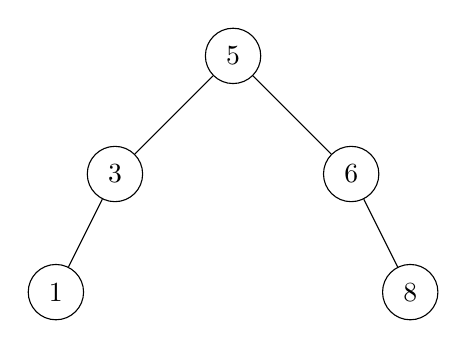
\begin{tikzpicture}[level distance=1.5cm,
                level 1/.style={sibling distance=3cm},
                level 2/.style={sibling distance=1.5cm},
                every node/.style = {minimum width = 2em, draw, circle}
                ]
                \node {5}
                    child {node {3}
                        child {node {1}}
                        child {edge from parent[draw = none]}
                    }
                    child {node {6}
                        child {edge from parent[draw = none]}
                        child {node {8}}
                    };
            \end{tikzpicture}
            \caption{Set the parent's reference to that node, in this case it's parents right reference equal to \lstinline|null|, to remove the node}
        \end{figure}
    \end{minipage}\\
    \vspace{0.25cm}\\
\end{frame}

\begin{frame}
    \frametitle{Case 2: Removing a Node with One Subtree}
    \vspace{0.1cm}\\
    \scalebox{0.8}{
    \begin{minipage}{0.32\textwidth}
        \centering
        \vspace{0.3cm}\\
        \begin{figure}[H]
            \begin{tikzpicture}[level distance=1.5cm,
                level 1/.style={sibling distance=3cm},
                level 2/.style={sibling distance=1.5cm},
                every node/.style = {minimum width = 2em, draw, circle},
                scale=0.7
                ]
                \node[fill=blue!70] {5}
                    child {node {3}
                        child {node {1}}
                        child {node {4}}
                    }
                    child {node[fill=!10!orange] {6}
                        child {edge from parent[draw = none]}
                        child {node {8}
                            child {node {7}}
                            child {node {9}}
                        }
                    };
            \end{tikzpicture}
            \caption{Find the node you want to remove (orange) and that node's parent (blue)}
            \label{fig:onesubtree-1}
        \end{figure}
    \end{minipage}}
    \pause
    \hfill
    \scalebox{0.8}{
    \begin{minipage}{0.32\textwidth}
        \centering
        \begin{figure}[H]
            \begin{tikzpicture}[level distance=1.5cm,
                level 1/.style={sibling distance=3cm},
                level 2/.style={sibling distance=1.5cm},
                every node/.style = {minimum width = 2em, draw, circle},
                scale=0.7
                ]
                \node[fill=blue!70] (P) {5}
                    child {node {3}
                        child {node {1}}
                        child {node {4}}
                    }
                    child {node[fill=!10!orange] (R) {6}
                        child {edge from parent[draw = none]}
                        child {node (C) {8}
                            child {node {7}}
                            child {node {9}}
                        }
                    };
                \draw (P) to [bend left=50] (C);

                % I can't figure out how to remove the edge from the tree so we're 
                % just going to use some "whiteout"
                \foreach \x in {0,...,4}
                \draw[thick, white!100] (P) to (R);
            \end{tikzpicture}
            \caption{Set \lstinline|parent.right| to the root of the node we want to remove's subtree.}
            \label{fig:onesubtree-2}
        \end{figure}
    \end{minipage}}
    \hfill
    \pause
    \scalebox{0.8}{
    \begin{minipage}{0.3\textwidth}
        \centering
        \vspace{0.95cm}\\
        \begin{figure}[H]
            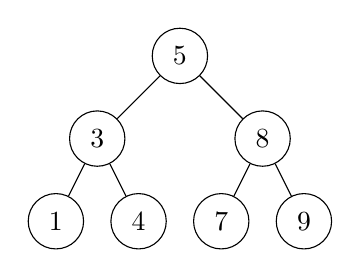
\begin{tikzpicture}[level distance=1.5cm,
                level 1/.style={sibling distance=3cm},
                level 2/.style={sibling distance=1.5cm},
                every node/.style = {minimum width = 2em, draw, circle},
                scale=0.7
                ]
                \node {5}
                    child {node {3}
                        child {node {1}}
                        child {node {4}}
                    }
                    child {node {8}
                        child {node {7}}
                        child {node {9}}
                    };
            \end{tikzpicture}
            \vspace{0.6cm}
            \caption{Set the node we  want to remove's reference to it's subtree is \lstinline|null|, thus removing it from the tree}
            \label{fig:onesubtree-3}
        \end{figure}
    \end{minipage}}
    \hfill
\end{frame}

\begin{frame}
    \frametitle{Case 3: Removing a Node with Two Subtrees}
    \vspace{0.25cm}\\
    \hfill
    \scalebox{0.7}{
    \begin{minipage}{0.32\textwidth}
        \centering
        \vspace{0.1cm}
        \begin{figure}[H]
            \begin{tikzpicture}[level distance=1.5cm,
                level 1/.style={sibling distance=2cm},
                level 2/.style={sibling distance=1.9cm},
                level 3/.style={sibling distance=1.0cm},
                every node/.style = {minimum width = 2em, draw, circle}
                ]
                \node {5}
                    child {node {3}}
                    child {node[fill=!10!orange] (R) {10}
                        child {node (C) {8}
                            child {node {7}}
                            child {node {9}}
                        }
                        child {node (C) {12}
                            child {node {11}}
                            child {node {13}}
                        }
                    };
            \end{tikzpicture}
            \caption{Find the node you want to remove (orange)}
            \label{fig:twosubtrees-0}
        \end{figure}
    \end{minipage}}
    \hfill
    \scalebox{0.7}{
    \begin{minipage}{0.32\textwidth}
        \centering
        \begin{figure}[H]
            \begin{tikzpicture}[level distance=1.5cm,
                level 1/.style={sibling distance=2cm},
                level 2/.style={sibling distance=1.9cm},
                level 3/.style={sibling distance=1.0cm},
                every node/.style = {minimum width = 2em, draw, circle}]
                \node (P) {5}
                    child {node {3}}
                    child {node[fill=!10!orange] (R) {11}
                        child {node {8}
                            child {node {7}}
                            child {node {9}}
                        }
                        child {node {12}
                            child {node[fill=red!70] (S) {11}}
                            child {node {13}}
                        }
                    };
                \draw[->, red, thick] (S) -- (R);
            \end{tikzpicture}
            \caption{Find the successor node (red) and copy the successor's value to the node we want to remove.}
            \label{fig:twosubtrees-1}
        \end{figure}
    \end{minipage}}
    \hfill
    \scalebox{0.7}{
    \begin{minipage}{0.3\textwidth}
        \centering
        \begin{figure}[H]
            \begin{tikzpicture}[level distance=1.5cm,
                level 1/.style={sibling distance=2cm},
                level 2/.style={sibling distance=1.9cm},
                level 3/.style={sibling distance=1.0cm},
                every node/.style = {minimum width = 2em, draw, circle}]
                \node (P) {5}
                    child {node {3}}
                    child {node[fill=!10!orange] (R) {11}
                        child {node {8}
                            child {node {7}}
                            child {node {9}}
                        }
                        child {node {12}
                            child {edge from parent[draw=none]}
                            child {node {13}}
                        }
                    };
            \end{tikzpicture}
            \caption{Call the removal method on the successor node.}
            \label{fig:twosubtrees-2}
        \end{figure}
    \end{minipage}}
    \hfill
    \vspace{0.25cm}\\
\end{frame}

\begin{frame}
	\frametitle{Removing a Node}
    \begin{minipage}{0.60\textwidth}
        \begin{algorithm}[H]
            \DontPrintSemicolon
            \tiny
            \SetKwFunction{FRemove}{Remove}
            \SetKwProg{Fn}{Function}{}{}
            \Fn{\FRemove{Val}}{
                root = Remove(Root, Val);
            }
            \vspace{0.2cm}
            \SetKwFunction{FRemove}{Remove}
            \SetKwProg{Fn}{Function}{}{}
            \Fn{\FRemove{Curr, Val}}{

                \If{curr $=$ null}{
                    \Return{null}\;
                }

                \begingroup
                \color{red}
                \If{Curr.val $<$ Val}{
                    Curr.right $\gets$ Remove(Curr.right, Val)\;
                } \ElseIf{Curr.val $>$ Val}{
                    Curr.left $\gets$ Remove(Curr.left, Val)\;
                } 
                \endgroup

                \Else {
                    \begingroup
                    \color{green}
                    \If{Curr.Left is NULL AND Curr.Right is NULL}{
                        \Return NULL
                    }
                    \endgroup
                    \begingroup
                    \color{blue}
                    \ElseIf{Curr.left is null}{
                    \Return Curr.right
                    }
                    \ElseIf{Curr.right is null}{
                        \Return Curr.left
                    }
                    \endgroup
                    \begingroup
                    \color{purple}
                    \Else {
                        MinNode $\gets$ Minimum(Curr.right)\;
                        Curr.data $\gets$ MinNode.data\;
                        Curr.right $\gets$ Remove(Curr.right, MinNode.data)\;
                        \Return Curr
                    }
                    \endgroup
                }
            }
    \end{algorithm}
    \end{minipage}
    \hfill
    \begin{minipage}{0.39\textwidth}
        \begin{itemize}
            \item \textbf{Step 1 (red): } Here we are recurring down the tree to search for the node we want to remove.
            \pause
            \item \textbf{Step 2: } Remove using cases
            \pause
            \begin{itemize}
                \item \textbf{Case 1 (green):} No subtree.
                \pause
                \item \textbf{Case 2 (blue):} One subtree.
                \pause
                \item \textbf{Case 3 (purple): } Both subtrees.
            \end{itemize}
        \end{itemize}
    \end{minipage}
\end{frame}


\begin{frame}
    \frametitle{Searching Unsorted Linear Data Structures vs Searching Binary Search Tree}
        \begin{minipage}{0.49\textwidth}
            \centering
            \begin{figure}[H]
                \scalebox{0.7}{
                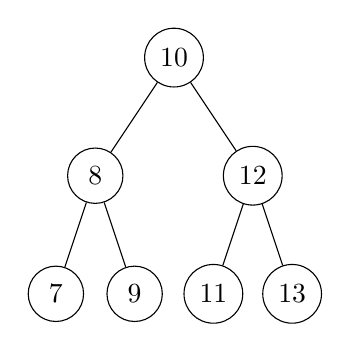
\begin{tikzpicture}[level distance=1.5cm,
                    level 1/.style={sibling distance=2cm},
                    level 2/.style={sibling distance=1.0cm},
                    every node/.style = {minimum width = 2em, draw, circle}]
                    \node (R) {10}
                        child {node {8}
                            child {node {7}}
                            child {node {9}}
                        }
                        child {node {12}
                            child {node (S) {11}}
                            child {node {13}}
                        };
                \end{tikzpicture}}
                \caption{Balanced BST}
            \end{figure}
    \end{minipage}
    \begin{minipage}{0.49\textwidth}
        \begin{figure}
            \scalebox{0.45}{
            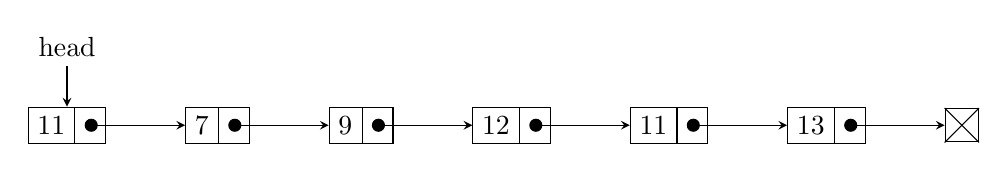
\begin{tikzpicture}[list/.style={rectangle split, rectangle split parts=2, draw, rectangle split horizontal}, >=stealth, start chain]

                \node[list,on chain] (A) {11};
                \node[list,on chain] (B) {7};
                \node[list,on chain] (C) {9};
                \node[list,on chain] (D) {12};
                \node[list,on chain] (E) {11};
                \node[list,on chain] (F) {13};


                \node[above of=A] (H) {head};

                \node[on chain,draw,inner sep=6pt] (N) {};
                \draw (N.north east) -- (N.south west);
                \draw (N.north west) -- (N.south east);


                \draw[*->] let \p1 = (A.two), \p2 = (A.center) in (\x1,\y2) -- (B);
                \draw[*->] let \p1 = (B.two), \p2 = (B.center) in (\x1,\y2) -- (C);
                \draw[*->] let \p1 = (C.two), \p2 = (C.center) in (\x1,\y2) -- (D);
                \draw[*->] let \p1 = (D.two), \p2 = (D.center) in (\x1,\y2) -- (E);
                \draw[*->] let \p1 = (E.two), \p2 = (E.center) in (\x1,\y2) -- (F);
                \draw[*->] let \p1 = (F.two), \p2 = (F.center) in (\x1,\y2) -- (N);

                \draw[->] (H) -- (A);


            \end{tikzpicture}}
            \caption{Linked List}
        \end{figure}
    \end{minipage}
    \vfill
    \scriptsize
    \begin{itemize}
        \item Searching a \textit{balanced} BST, search is $O(log_2(n))$ where $n$ is the number of nodes in the tree.
        \item Recall, searching a linked list is $(log_2(n))$ where $n$ is the number of nodes in the list.
    \end{itemize}

\end{frame}

\begin{frame}
    \frametitle{The Issue of Unbalanced Binary Search Trees}
    \begin{minipage}{0.49\textwidth}
        \centering
        \begin{figure}[H]
            \scalebox{0.7}{
            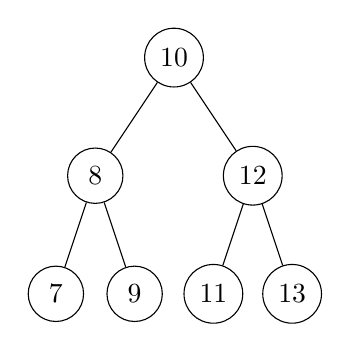
\begin{tikzpicture}[level distance=1.5cm,
                level 1/.style={sibling distance=2cm},
                level 2/.style={sibling distance=1.0cm},
                level 3/.style={sibling distance=.75cm},
                every node/.style = {minimum width = 2em, draw, circle}]
                \node (R) {10}
                    child {node {8}
                        child {node {7}}
                        child {node {9}}
                    }
                    child {node {12}
                        child {node (S) {11}}
                        child {node {13}}
                    };
            \end{tikzpicture}}
            \caption{Balanced BST}
        \end{figure}
    \end{minipage}
    \hfill
    \begin{minipage}{0.49\textwidth}
        \centering
        \begin{figure}[H]
            \scalebox{0.7}{
            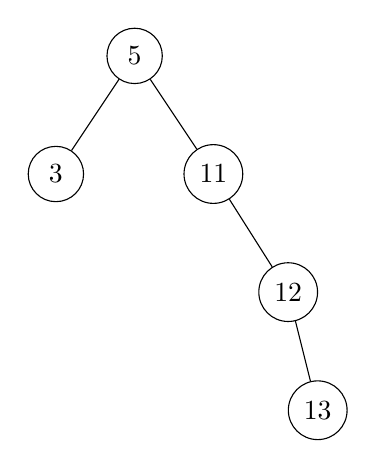
\begin{tikzpicture}[level distance=1.5cm,
                level 1/.style={sibling distance=2cm},
                level 2/.style={sibling distance=1.9cm},
                level 3/.style={sibling distance=.75cm},
                every node/.style = {minimum width = 2em, draw, circle}]
                \node (P) {5}
                    child {node {3}}
                    child {node (R) {11}
                            child {edge from parent[draw=none]}
                        child {node {12}
                            child {edge from parent[draw=none]}
                            child {node {13}}
                        }
                    };
            \end{tikzpicture}}
            \caption{Unbalanced BST}
        \end{figure}
    \end{minipage}
    \vfill
    \scriptsize
    \begin{itemize}
        \item For \textit{balanced} BST, search is $O(log_2(n))$ where $n$ is the number of nodes in the tree.
        \item For \textit{unbalanced} BST, search is $O(h)$ where $h$ is the height of the tree.
        \item We want to make sure our tree remains balanced when we insert/delete but this can't be done with traditional BST.
        \item \textbf{Next week:} AVL self balancing trees
    \end{itemize}
\end{frame}


\end{document}
